\section{Результаты}
\label{sec:conclusion-future}
%%
В рамках работы была реализована стадия компиляции, направленная на деление структур по типам, с целью их последующих векторизаций и разложений по регистрам. Разработан алгоритм с делением структур неограниченной вложенности. Предложен способ замены инструкций с сохранением корректности работы программы.

Опорными тестами были программы открытого стека рендеринга Intel(OSPray, Embree). На них происходило тестирование корректности алгоритма и отслеживание влияния на производительность. На Рис.~\ref{fig:results_name} и Рис.~\ref{fig:results_pure} показан прирост скорости работы приложений при различных SIMD и на различных платформах. На первых тестах, где структуры не были использованы, нет прироста производительности, однако с ростом сложности программ и с ростом использования структур наблюдается прирост производительности вплоть до 88\%.

\begin{figure}[h]
    \centering
    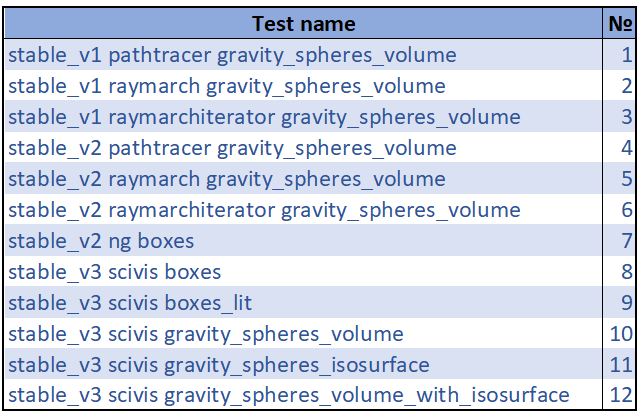
\includegraphics[scale=0.55]{Images/results_name.png}
    \caption{Названия тестов.}
    \label{fig:results_name}
\end{figure}

\begin{figure}[h]
    \centering
    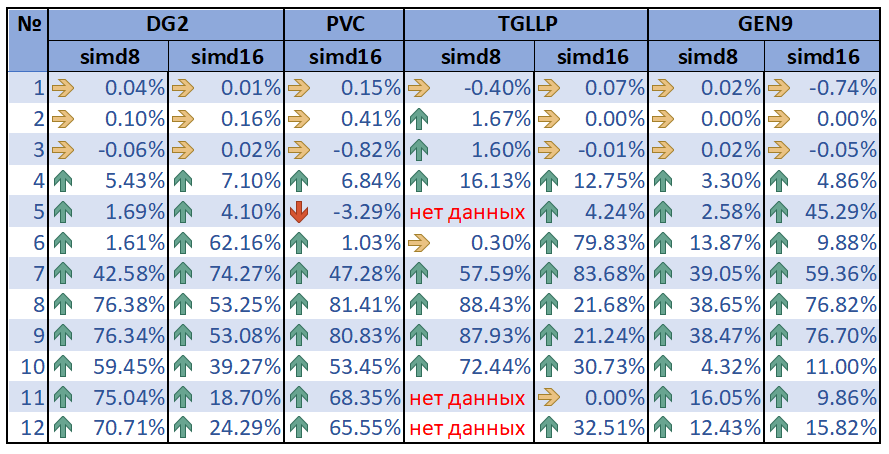
\includegraphics[scale=0.54]{Images/results_pure.png}
    \caption{Результаты работы.}
    \label{fig:results_pure}
\end{figure}

Дальнейшие улучшения могут быть достигнуты следующими дополнениями:
\begin{itemize}
    \item Поддержка использований указателей.
    \item Поддержка пользовательских функций.
    \item Поддержка деления векторов и массивов структур.
    \item Ограничение на деление структур с использованием эвристик.
\end{itemize}